\documentclass[a4paper]{article} % Formato de Plantilla  que voy a utilizar

\usepackage[utf8]{inputenc} % Que me interprete todos los caracteres
\usepackage[spanish]{babel} % Se trabaja en español
\usepackage[margin=2cm, top=2cm, includefoot]{geometry}
\usepackage{graphicx} % Para la insercion de imagenes
\usepackage[table,xcdraw]{xcolor} % Para la deteción de colores
\usepackage[most]{tcolorbox} % Para la inserción de cuadros en la portada
\usepackage{fancyhdr} % Definir el estilo de la página
\usepackage{multirow} % Para centrar las palabras en las tablas
\usepackage[hidelinks]{hyperref} % Gestión de hipervinculos
\usepackage{listings} % Para la inserción de código en el documento
\usepackage{parskip} % Arreglo de la tabulación en el documento
\usepackage[figurename=Figura]{caption} % Cambiar el nombre del caption de las fotos
\usepackage{smartdiagram} % Para la inserción de diagramas
\usepackage{zed-csp} % Para la inserción de esquemas
\usepackage{pdfpages} % Para insertar PDF, en mi caso de Portada
\usepackage{tikz} % Para escribir encima del pdf
\usepackage{tabularray}

% Declaración de colores
\definecolor{blackPortada}{HTML}{000000} 
\definecolor{greenPortada}{HTML}{75d14f}
\definecolor{critico}{HTML}{b00505}
\definecolor{table1}{HTML}{2c83a8} % Color definido para la tabla1
\definecolor{lima}{HTML}{44f205} % Color para la tabla2 que son los Activos dentro del Alcance
\definecolor{gris}{HTML}{cdd1cf} % Color para la tabla2 que son los Activos dentro del Alcance

% Declaración de variables
\newcommand{\logoPortada}{images/hackthebox.png} % Logo de la empresa
%\newcommand{\moduloName}{Write-Up Topology} % Nombre de los modulos, se cambia siempre por otro Name
\newcommand{\logoModulo}{images/Topology.png} % Logo de la máquina
\newcommand{\mylogo}{images/maa.png} % Logo de la máquina
\newcommand{\starDate}{9 de Febrero del 2024} % Fecha 

% Adicionales
\addto\captionsspanish{\renewcommand{\contentsname}{Índice}} % Cambio el formato del Índice
\setlength{\headheight}{40.2pt} % Espacio de la linea para insertar imagen en el encabezado
\pagestyle{fancy} % Estilo de la página
\fancyhf{} % Estilo de la página 
\lhead{\includegraphics[width=5cm]{\logoPortada}} % Inserto el logo de la empresa a la LEFT en el encabezado
\rhead{\includegraphics[height=1.25cm]{\logoModulo}} % Inserto el logo del modulo a la RIGHT en el encabezado
\renewcommand{\headrulewidth}{3pt} % Defino la anchura de la barra del encabezado
\renewcommand{\headrule}{\hbox to\headwidth{\color{blackPortada}\leaders\hrule height \headrulewidth\hfill}} % Definimos el color de la barra del encabezado
\cfoot{\href{https://0mariano.github.io}{\includegraphics[height=1.25cm]{\mylogo}}} % Inserto my logo en el LEFT en el pie de página
\renewcommand{\footrulewidth}{3pt} % Defino la anchura de la barra del encabezado
\renewcommand{\footrule}{\hbox to\headwidth{\color{blackPortada}\leaders\hrule height \footrulewidth\hfill}} % Definimos el color de la barra del pie de página
\renewcommand{\lstlistingname}{Código} % Cambio de nombre del caption de los códigos

\definecolor{codegreen}{rgb}{0,0.6,0} % Para insertar código
\definecolor{codegray}{rgb}{0.5,0.5,0.5}
\definecolor{codepurple}{rgb}{0.58,0,0.82}
\definecolor{backcolour}{rgb}{0.95,0.95,0.92}

\lstdefinestyle{mystyle}{
backgroundcolor=\color{backcolour},
commentstyle=\color{codegreen},
keywordstyle=\color{magenta},
numberstyle=\tiny\color{codegray},
stringstyle=\color{codepurple},
basicstyle=\ttfamily\footnotesize,
breakatwhitespace=false, 
frame=single,
breaklines=true,
captionpos=b,
keepspaces=true, 
numbers=left,
numbersep=5pt, 
showspaces=false, 
showstringspaces=false,
showtabs=false, 
 tabsize=2
}

\lstset{style=mystyle} % Termina la sintaxis para insertar código

% Comienzo del documento
\begin{document}
\rfoot{\begin{minipage}[b][1cm][c]{0.5\textwidth}\raggedleft\textbf{\thepage}\end{minipage}} % Numeros de páginas
\lfoot{\begin{minipage}[b][1cm][c]{0.5\textwidth}\href{https://www.linkedin.com/in/mariano-alfonso-667a60226}{\textbf{MARIANO ALFONSO}}\end{minipage}} % Autor
% Creación de portada
\begin{titlepage}
\begin{tikzpicture}[remember picture,overlay]
\fill ([yshift=-50cm]current page.south) rectangle (current page.north);
\node at (current page.center) {\includegraphics[width=\paperwidth,height=\paperheight]{Portada.pdf}}; % Incluyo el PDF de la Portada como imagen
\node[anchor=north,text width=15cm,align=center] at ([yshift=-20cm]current page.north) {
\begin{tcolorbox}[enhanced,attach boxed title to top center={yshift=-3mm,yshifttext=-1mm},
colback=blue!5!white,colframe=blue!75!black,colbacktitle=red!80!black,
title=\href{https://0mariano.github.io}{\textbf{\color{white}https://0mariano.github.io}},fonttitle=\bfseries,
 boxed title style={size=small,colframe=red!50!black} ]
\centering
\bfseries En este \underline{Write-Up}, no solo compartiré los pasos para resolver la máquina Topology de la plataforma \underline{\href{https://www.hackthebox.com}{\textbf{\color{black}HackTheBox}}}, sino que también mi objetivo es fomentar la colaboración y el intercambio de conocimientos dentro de la comunidad de la \underline{CiberSeguridad}, \underline{Pentesting}, \underline{Hacking Ético}.
\end{tcolorbox}
\vfill % Estiro y aprovecho toda la hoja
\par\vspace{1cm}
{\large \bfseries \starDate\par}
\vfill % Estiro y aprovecho toda la hoja
 };
\end{tikzpicture}
%\includepdf{Portada.pdf} % Inserto un pdf como portada
\end{titlepage}

% -----------------------------------------------------------------------------------------

% Comienzo del TOC (Table of Contens)
\clearpage
\tableofcontents
\clearpage
 
% -----------------------------------------------------------------------------------------

\section{Introducción}
En este \underline{Write-Up}, no solo compartiré los pasos para resolver la máquina Topology de la plataforma \underline{\href{https://www.hackthebox.com}{\textbf{\color{black}HackTheBox}}}, sino que también mi objetivo es fomentar la colaboración y el intercambio de conocimientos dentro de la comunidad de la \textbf{CiberSeguridad}, \textbf{Pentesting}, \textbf{Hacking Ético}.\par

\href{https://app.hackthebox.com/machines/Topology}{\textbf{\color{black}Topology}} se trata de una máquina basada en el Sistema Operativo Linux, donde a través de \textbf{Local File Inclusion} (LFI) via \textbf{LaTeX Injection} se obtiene un archivo que contiene \textbf{credenciales} que luego se utilizan para entablar conexión por \textbf{SSH}. Finalmente, para la \textbf{escalada de privilegios}, se debe crear un archivo con \textbf{extensión .plt} para el programa \textbf{gnuplot}, con el fin de convertir la BASH en permisos \textbf{SUID}.\par

    \subsection{Alcance}
    El alcance de esta máquina fue definida como la siguiente.\par\vspace{0.2cm}
        \begin{table}[ht]
        \centering
        \begin{tabular}{|c|c|c|}
            \hline
            \multicolumn{3}{|>{\columncolor{table1}}c|}{{\textcolor{white}{Alcance de la máquina}}} \\
            \hline
            \multicolumn{1}{|>{\columncolor{lima}}c|}{Servidor Web / Direcciónes IPs / Hosts / URLs} & \multicolumn{1}{|>{\columncolor{lima}}c|}{Descripción} & \multicolumn{1}{|>{\columncolor{lima}}c|}{Subdominios} \\
            \hline
            \multicolumn{1}{|>{\columncolor{gris}}c|}{10.129.16.121} & \multicolumn{1}{|>{\columncolor{gris}}c|}{Dirección IP de la máquina Topology} & \multicolumn{1}{|>{\columncolor{gris}}c|}{Todos} \\
            \hline
        \end{tabular}
        \captionsetup{labelfont=bf} % Caption de la tabla en color negrita
        \caption{Alcance pactado.}
        \end{table}\par\vspace{0.2cm}

    \subsection{Metodologia Aplicada}
        \begin{itemize}\itemsep1.25pt
        \item[$\bullet$] Enfoque de prueba: En el proceso de pruebas de seguridad, se optó por un enfoque gray-box, lo que significó que se tenía un nivel de acceso parcial a la infraestructura y el sistema objetivo.\itemsep3.5pt
        \item[$\bullet$] Las etapas aplicadas para esta auditoria fueron las siguientes:\itemsep3.5pt
        \end{itemize}\par\vspace{0.5cm}
    
    \begin{figure}[h] % Con "h" indico que coloque la imagen abajo del texto
        \begin{center}
            \smartdiagramset{
            set color list={greenPortada,orange,red,critico},
            priority arrow width=2cm,
            priority arrow height advance=2.25cm
            }
            \smartdiagram[priority descriptive diagram]{Reconocimiento \texttt{{-}} Enumeración,Análisis de Vulnerabilidades,Explotación,Escalada de Privilegios}
        \end{center}
    \captionsetup{labelfont=bf} % Caption de la tabla en color negrita
    \caption{Etapas aplicadas al pentest.}   
    \end{figure}
    
\vspace{5cm}
    
\section{Reconocimiento - Enumeración}

    \subsection{Uso de la Herramienta Nmap}

    \vspace{0.2cm}

    Primeramente realizamos un escaneo con ayuda de la herramienta {\href{https://nmap.org}{\textbf{\color{black}Nmap}}} en búsqueda de puertos abiertos.

    \vspace{0.2cm}

    \captionsetup[lstlisting]{labelfont=bf} % Caption del código en color negrita
    \begin{lstlisting}[language=C, caption=Primer escaneo., aboveskip=0.5cm]
         
                        nmap -p- --open -sV --min-rate 5000 10.129.16.121
    \end{lstlisting}
    
    \begin{table}[ht]
        \centering
        \begin{tabular}{|c|c|}
        \hline
        {\color[HTML]{3B00F6} \textbf{Parámetro}} & {\color[HTML]{3B00F6} \textbf{Descripción}}                                         \\ \hline
        \textbf{-p-}                              & Escanea los 65535 puertos.                                                          \\ \hline
        \textbf{\texttt{{-}{-}open}}                          & Muestra solo los puertos abiertos.                                                  \\ \hline
        \textbf{-sV}                              & Determina la versiones de los servicios que se ejecutan en los puertos encontrados. \\ \hline
        \textbf{\texttt{{-}{-}min-rate 5000}}                  & Establece la velocidad mínima de envío de paquetes a 5000 paquetes por segundo.     \\ \hline
        \end{tabular}
    \captionsetup{labelfont=bf} % Caption de la tabla en color negrita
    \caption{Definición de parámetros de nmap utilizados en el primer escaneo.}
    \end{table}

    El resultado que nos arrojó este primer escaneo fue que la máquina tiene el puerto \textbf{22} que pertenece al servicio \textit{SSH} y el puerto \textbf{80} que pertenece al protocolo \textit{HTTP}.

    \begin{figure}[h] % Con "h" indico que coloque la imagen abajo del texto
        \begin{center}
        \setlength{\fboxsep}{0.2em} % Ajustar la distancia del borde interno
        \fbox{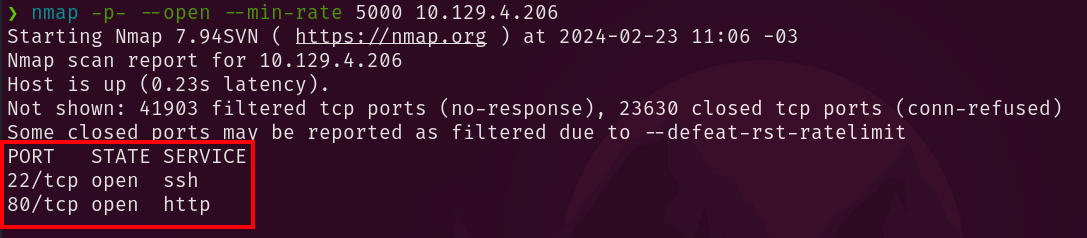
\includegraphics[width=1\textwidth]{images/nmap_1.png}} % Utilizo \fbox para crear un borde alrededor de la imagen
        \end{center}
        \captionsetup{labelfont=bf} % Caption de la tabla en color negrita
        \caption{Resultado del primer escaneo.}
    \end{figure}
    
    Se procedió a realizar otro escaneo con los scripts default de nmap, también especificando la versión nuevamente.

    \vspace{0.2cm}

    \captionsetup[lstlisting]{labelfont=bf} % Caption del código en color negrita
    \begin{lstlisting}[language=C, caption=Segundo escaneo., aboveskip=0.5cm]
         
                              nmap -sC -sV -p22,80 10.129.16.121
    \end{lstlisting}

    \begin{table}[ht]
        \centering
        \begin{tabular}{|c|c|}
        \hline
        {\color[HTML]{3B00F6} \textbf{Parámetro}} & {\color[HTML]{3B00F6} \textbf{Descripción}}                                         \\ \hline
        \textbf{-sC}                              & Realiza un escaneo con los scripts por defecto.                                                          \\ \hline
        \textbf{-sV}                              & Determina la versiones de los servicios que se ejecutan en los puertos encontrados. \\ \hline
        \textbf{-p}                  & Especifica los puertos que se escanearán.     \\ \hline
        \end{tabular}
    \captionsetup{labelfont=bf} % Caption de la tabla en color negrita
    \caption{Definición de parámetros de nmap utilizados en el segundo escaneo.}
    \end{table}

    \vspace{4cm}

    Lo único interesante que obtenemos, es el título de la página web \textbf{Miskatonic University \texttt{|} Topology Group}.

    \begin{figure}[h] % Con "h" indico que coloque la imagen abajo del texto
        \begin{center}
        \setlength{\fboxsep}{0.2em} % Ajustar la distancia del borde interno
        \fbox{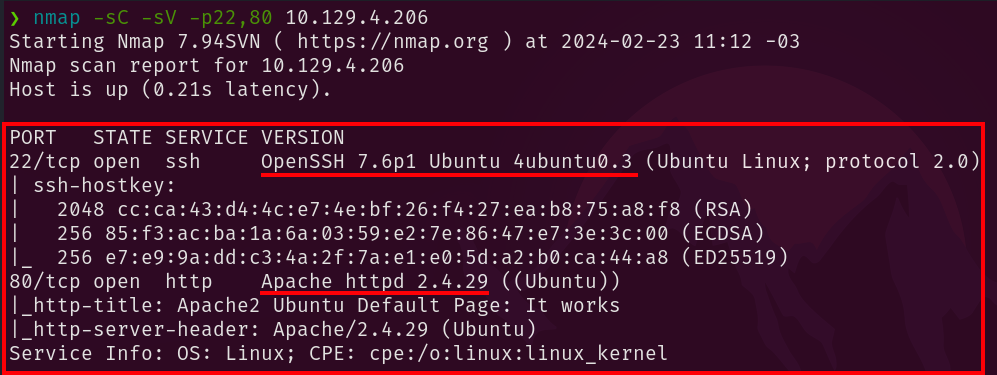
\includegraphics[width=1\textwidth]{images/nmap_2.png}} % Utilizo \fbox para crear un borde alrededor de la imagen
        \end{center}
        \captionsetup{labelfont=bf} % Caption de la tabla en color negrita
        \caption{Resultado del segundo escaneo.}
    \end{figure}
    
    \subsection{Aplicación Web}

    \vspace{0.2cm}

    Luego del segundo escaneo, se ingresó a la aplicación web, donde en el código fuente se encontró un subdominio \textbf{http://latex.topology.htb/equation.php}

    \begin{figure}[h] % Con "h" indico que coloque la imagen abajo del texto
        \begin{center}
        \setlength{\fboxsep}{0.2em} % Ajustar la distancia del borde interno
        \fbox{\includegraphics[width=0.99\textwidth]{images/código-fuente.png}} % Utilizo \fbox para crear un borde alrededor de la imagen
        \end{center}
        \captionsetup{labelfont=bf} % Caption de la tabla en color negrita
        \caption{Código fuente.}
    \end{figure}

    \vspace{4cm}

    Antes de ingresar al subdominio, se agregó el mismo al archivo \textbf{/etc/hosts}

    \captionsetup[lstlisting]{labelfont=bf} % Caption del código en color negrita
    \begin{lstlisting}[language=c, caption=Agregando subdominio al archivo /etc/hosts, aboveskip=0.5cm]
        
    sudo nano /etc/hosts
          
    10.129.16.121 latex.topology.htb
    \end{lstlisting}

\vspace{20cm}

\section{Análisis de Vulnerabilidades}
Al ingresar al subdominio, vemos que cosiste en una generador de ecuaciones mediante sintaxis en LaTeX.

\begin{figure}[h] % Con "h" indico que coloque la imagen abajo del texto
    \begin{center}
    \setlength{\fboxsep}{0.2em} % Ajustar la distancia del borde interno
    \fbox{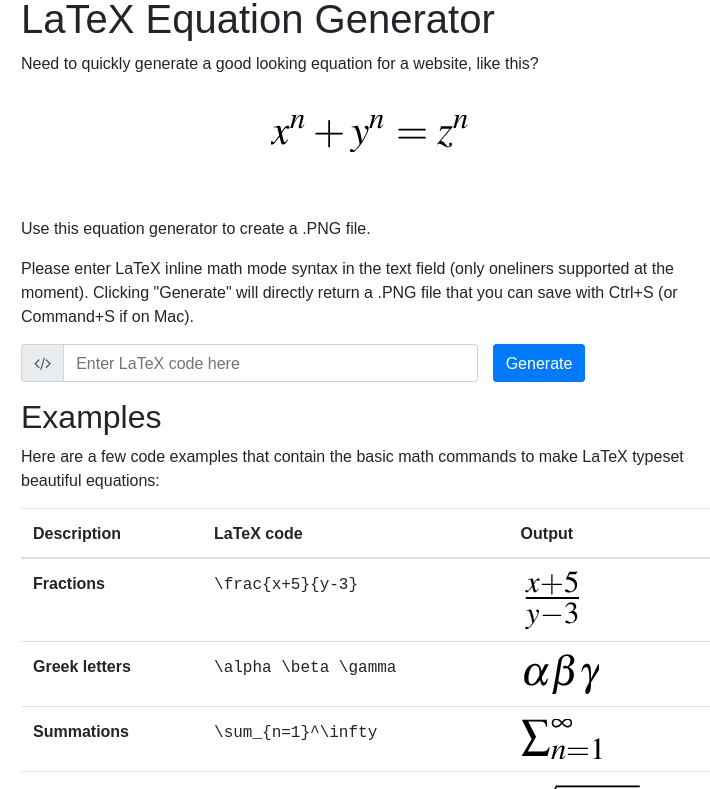
\includegraphics[width=0.88\textwidth]{images/Latex-equation.png}} % Utilizo \fbox para crear un borde alrededor de la imagen
    \end{center}
    \captionsetup{labelfont=bf} % Caption de la tabla en color negrita
    \caption{Aplicación web.}
\end{figure}

\vspace{5cm}

Realizamos un \textbf{PoC}, para ver más en detalle la funcionalidad de la aplicación web.

\begin{figure}[h] % Con "h" indico que coloque la imagen abajo del texto
    \begin{center}
    \setlength{\fboxsep}{0.2em} % Ajustar la distancia del borde interno
    \fbox{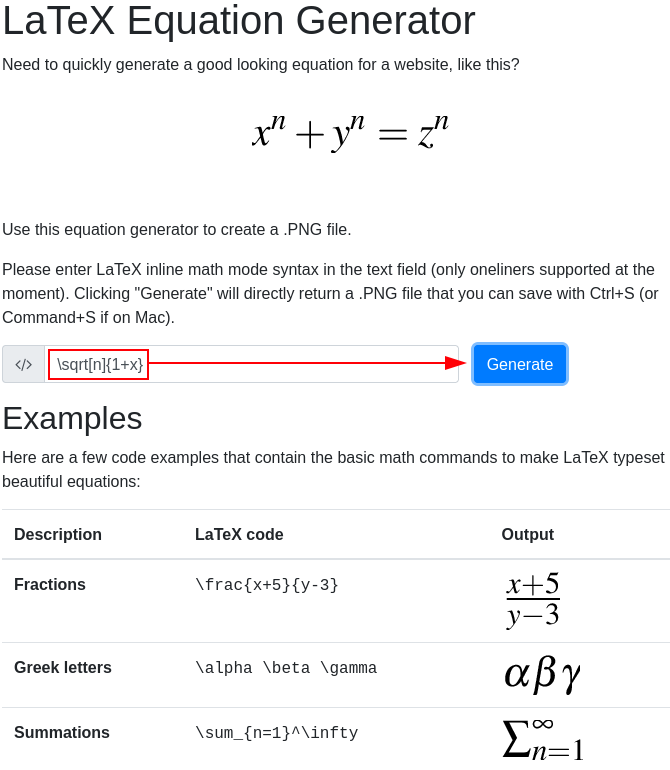
\includegraphics[width=0.88\textwidth]{images/PoC_1.png}} % Utilizo \fbox para crear un borde alrededor de la imagen
    \end{center}
    \captionsetup{labelfont=bf} % Caption de la tabla en color negrita
    \caption{Realizando PoC.}
\end{figure}

\vspace{6cm}

Una vez que enviamos el comando de LaTeX para generar la ecuación, nos envia a una ruta con la ecuación generada en formaato de imagen.

\begin{figure}[h] % Con "h" indico que coloque la imagen abajo del texto
    \begin{center}
    \setlength{\fboxsep}{0.2em} % Ajustar la distancia del borde interno
    \fbox{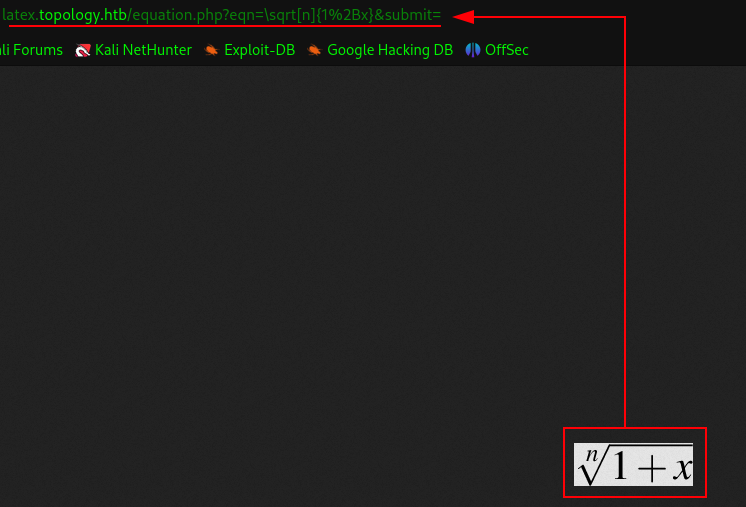
\includegraphics[width=1\textwidth]{images/PoC_resultado.png}} % Utilizo \fbox para crear un borde alrededor de la imagen
    \end{center}
    \captionsetup{labelfont=bf} % Caption de la tabla en color negrita
    \caption{Ecuación generada.}
\end{figure}

Muy interesante el funcionamiento de la aplicación y de como se genera la ecuación.\par

\vspace{8cm}

    \subsection{Local File Inlcusion (LFI) via LaTeX Injection}

    \vspace{0.2cm}
    
    Al entender como funciona la aplicación, se me ocurrió realizar una prueba que consiste en incluir el archivo \textbf{/etc/passwd}, ingresando código de LaTeX arbitrario.\par

    Para realizar esta prueba se utilizó en siguiente recurso \href{https://book.hacktricks.xyz/v/es/pentesting-web/formula-csv-doc-latex-ghostscript-injection}{\textbf{\color{blue}https://book.hacktricks.xyz/v/es/pentesting-web/formula-csv-doc-latex-ghostscript-injection}} de \href{https://book.hacktricks.xyz}{\textbf{\color{red}HackTricks}}

    Realicé una prueba para incluir el archivo \textbf{/etc/passwd} con el siguiente comando \textbf{\$\texttt{\string\input}/etc/passwd\$}

    \begin{figure}[h] % Con "h" indico que coloque la imagen abajo del texto
        \begin{center}
        \setlength{\fboxsep}{0.2em} % Ajustar la distancia del borde interno
        \fbox{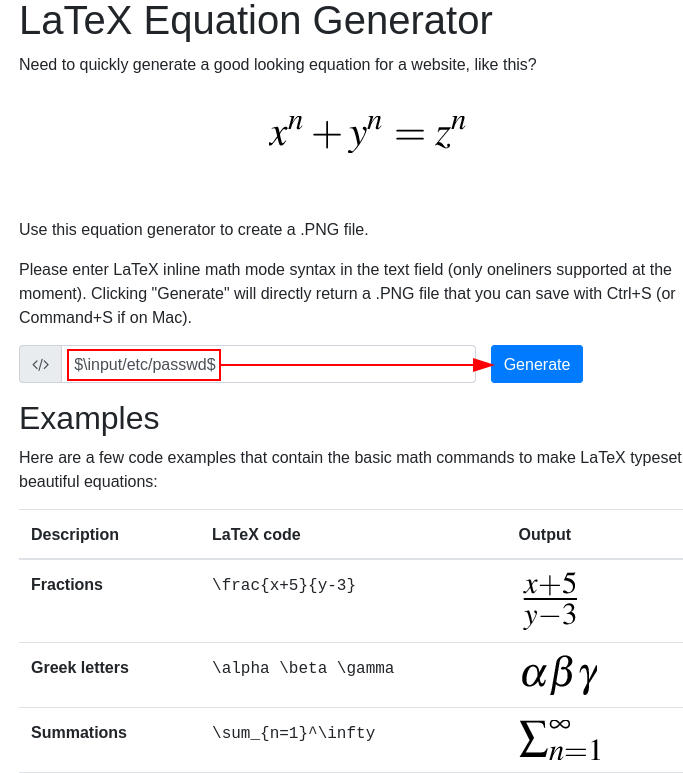
\includegraphics[width=0.9\textwidth]{images/Latex-Injection.png}} % Utilizo \fbox para crear un borde alrededor de la imagen
        \end{center}
        \captionsetup{labelfont=bf} % Caption de la tabla en color negrita
        \caption{Comando ingresado.}
    \end{figure}

    \vspace{5cm}

    Como resultado la apliación detecta que se están ingresando comandos arbitrarios.

    \begin{figure}[h] % Con "h" indico que coloque la imagen abajo del texto
        \begin{center}
        \setlength{\fboxsep}{0.2em} % Ajustar la distancia del borde interno
        \fbox{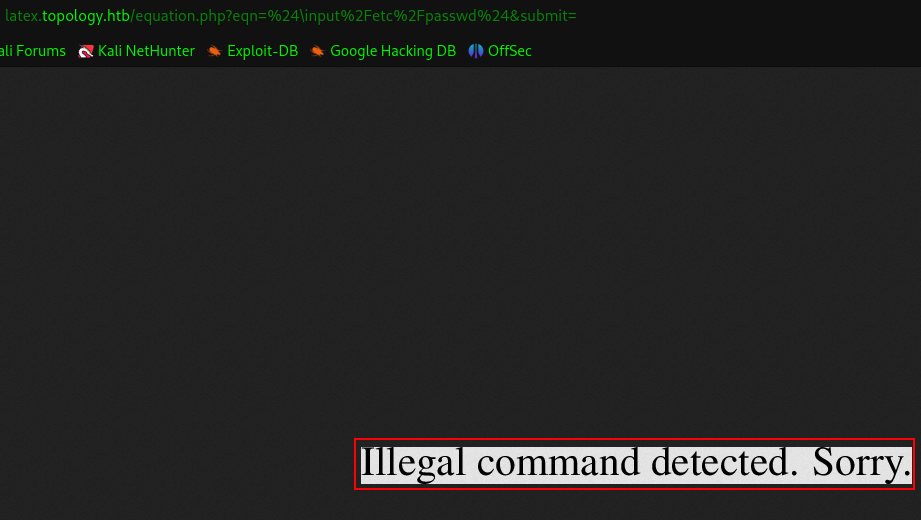
\includegraphics[width=0.9\textwidth]{images/Latex-Injection-Resultado.png}} % Utilizo \fbox para crear un borde alrededor de la imagen
        \end{center}
        \captionsetup{labelfont=bf} % Caption de la tabla en color negrita
        \caption{Imagen generada.}
    \end{figure}

    \vspace{14cm}

    Después de varios intentos, el comando que me funcionó para obtener lectura del archivo \textbf{/etc/passwd}, fue el siguiente:

    \begin{figure}[h] % Con "h" indico que coloque la imagen abajo del texto
        \begin{center}
        \setlength{\fboxsep}{0.2em} % Ajustar la distancia del borde interno
        \fbox{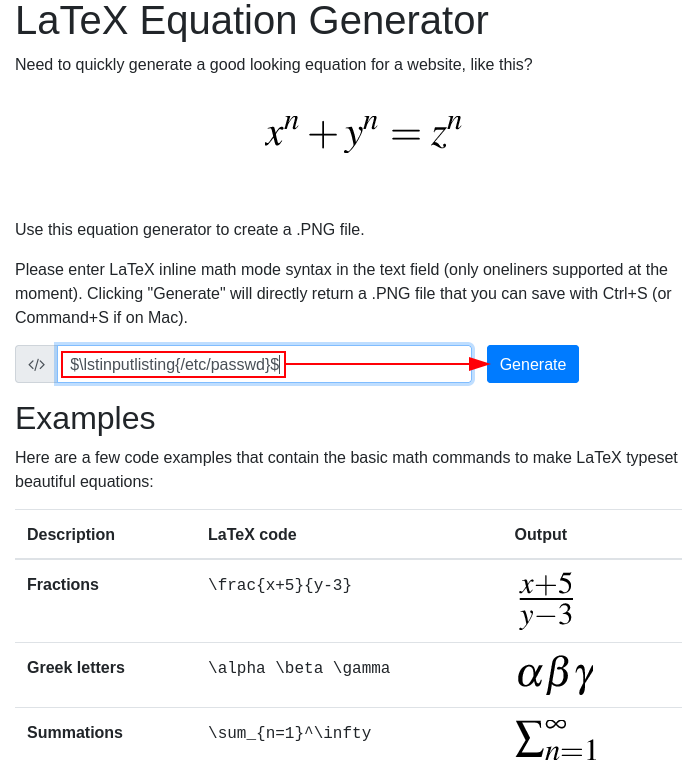
\includegraphics[width=0.9\textwidth]{images/Latex-Injection_2.png}} % Utilizo \fbox para crear un borde alrededor de la imagen
        \end{center}
        \captionsetup{labelfont=bf} % Caption de la tabla en color negrita
        \caption{Comando útil.}
    \end{figure}

    \vspace{6cm}

    Como resultado genera la imagen del archivo \textbf{/etc/passwd}

    \begin{figure}[h] % Con "h" indico que coloque la imagen abajo del texto
        \begin{center}
        \setlength{\fboxsep}{0.2em} % Ajustar la distancia del borde interno
        \fbox{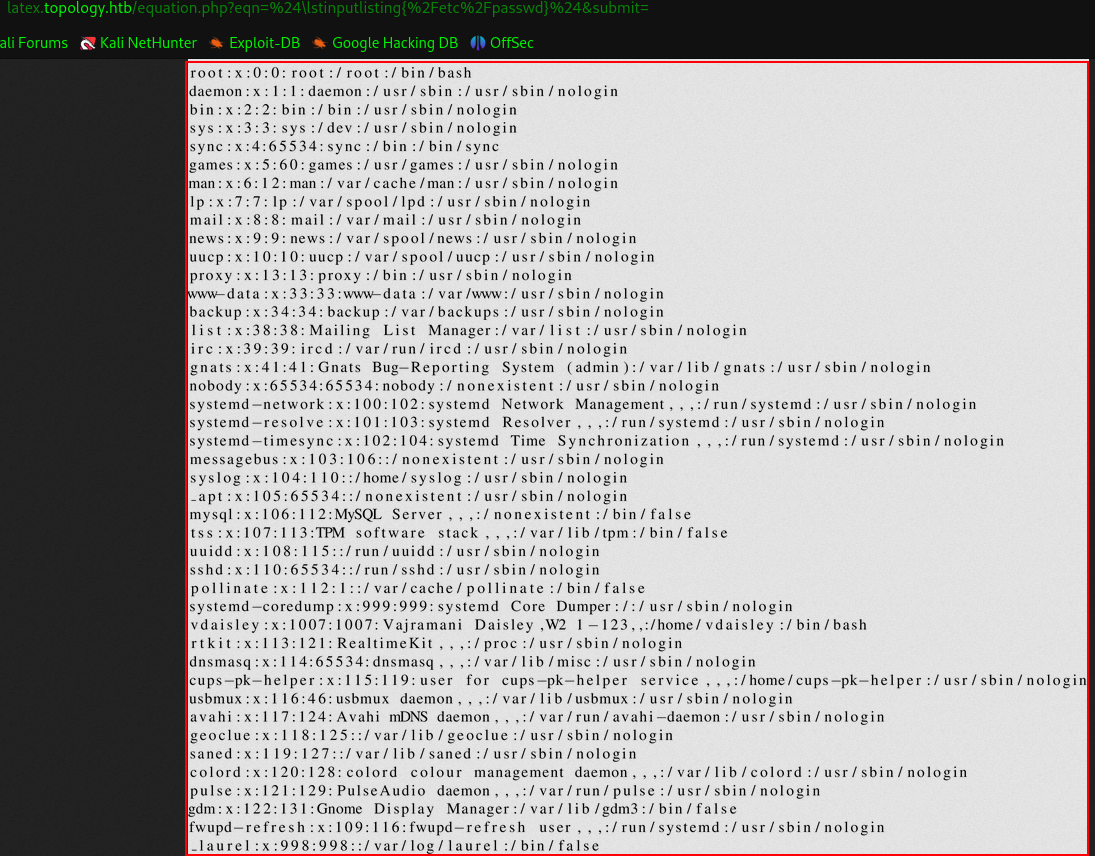
\includegraphics[width=1\textwidth]{images/Latex-Injection_2_Resultado.png}} % Utilizo \fbox para crear un borde alrededor de la imagen
        \end{center}
        \captionsetup{labelfont=bf} % Caption de la tabla en color negrita
        \caption{Archivo /etc/passwd}
    \end{figure}

\vspace{8cm}

\section{Explotación}

    \subsection{Enumeración de Archivos del Sistema}

    \vspace{0.2cm}

    Al obtener lectura del archivo, se confirma que la aplicación web es vulnerable a \textbf{Local File Inclusion} via \textbf{LaTeX Injection}.

    Utilizaremos esta vulnerabilidad para conseguir posibles datos que nos interesen o sean útiles. 

    Como la app web tiene un servidor web apache, procedemos a leer el archivo de configuración predeterinado del servidor web, que se encuentra en esta ruta \textbf{/etc/apache2/sites-available/000-default.conf}

    \begin{figure}[h] % Con "h" indico que coloque la imagen abajo del texto
        \begin{center}
        \setlength{\fboxsep}{0.2em} % Ajustar la distancia del borde interno
        \fbox{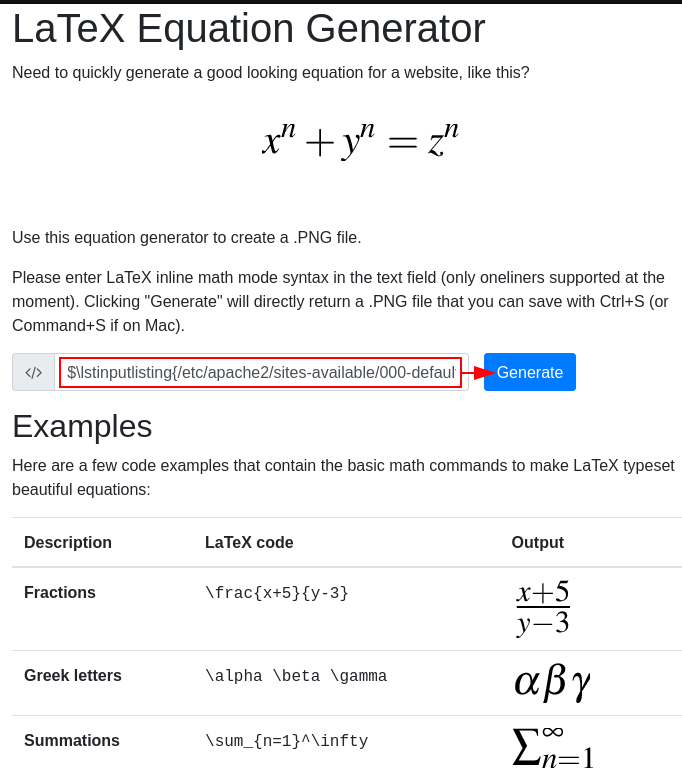
\includegraphics[width=0.9\textwidth]{images/comando-archivo-config.png}} % Utilizo \fbox para crear un borde alrededor de la imagen
        \end{center}
        \captionsetup{labelfont=bf} % Caption de la tabla en color negrita
        \caption{Comando para obtener lectura del archivo de configuración.}
    \end{figure}

    \vspace{3cm}

    Obtenemos el resultado, donde se aprecia la ruta de la landing page de la universidad y las demas rutas de los aplicativos.

    \begin{figure}[h] % Con "h" indico que coloque la imagen abajo del texto
        \begin{center}
        \setlength{\fboxsep}{0.2em} % Ajustar la distancia del borde interno
        \fbox{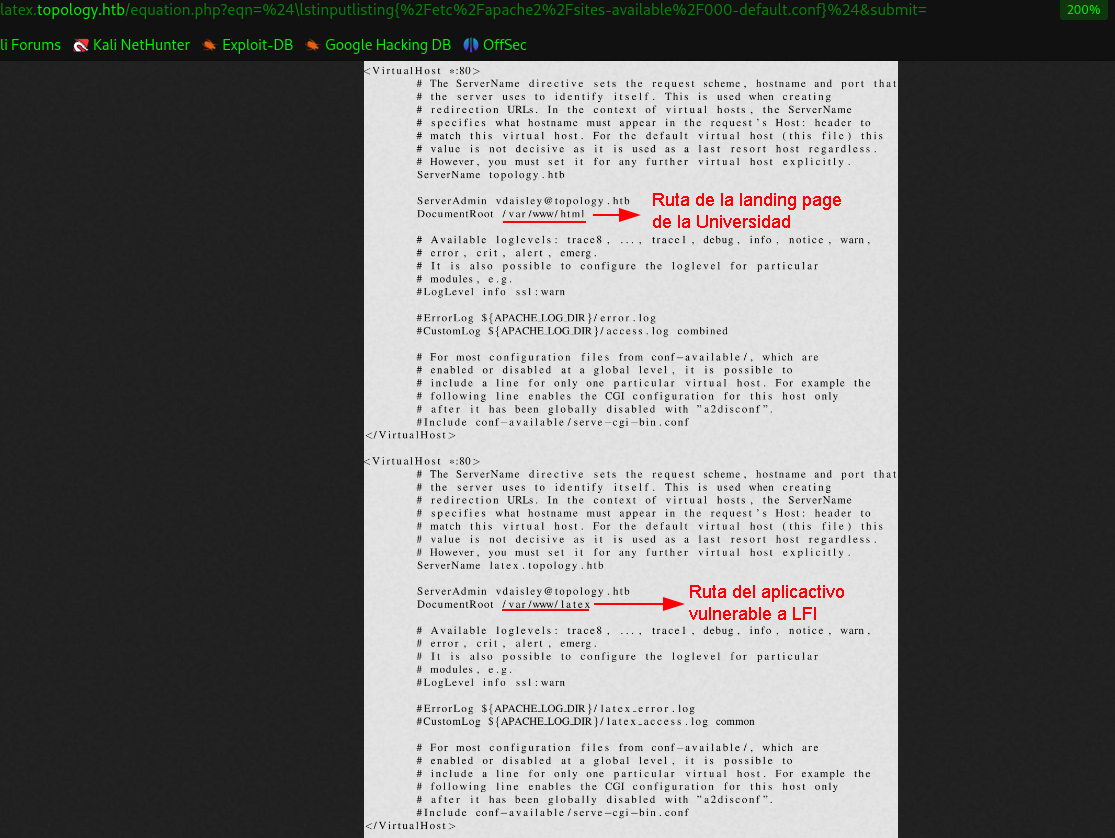
\includegraphics[width=1\textwidth]{images/archivo-cofig_1.png}} % Utilizo \fbox para crear un borde alrededor de la imagen
        \end{center}
        \captionsetup{labelfont=bf} % Caption de la tabla en color negrita
        \caption{Aplicativos con sus respectivas rutas.}
    \end{figure}

    \vspace{10cm}

    Además se encuentran otros aplicativos con sus respectivas rutas.

    \begin{figure}[h] % Con "h" indico que coloque la imagen abajo del texto
        \begin{center}
        \setlength{\fboxsep}{0.2em} % Ajustar la distancia del borde interno
        \fbox{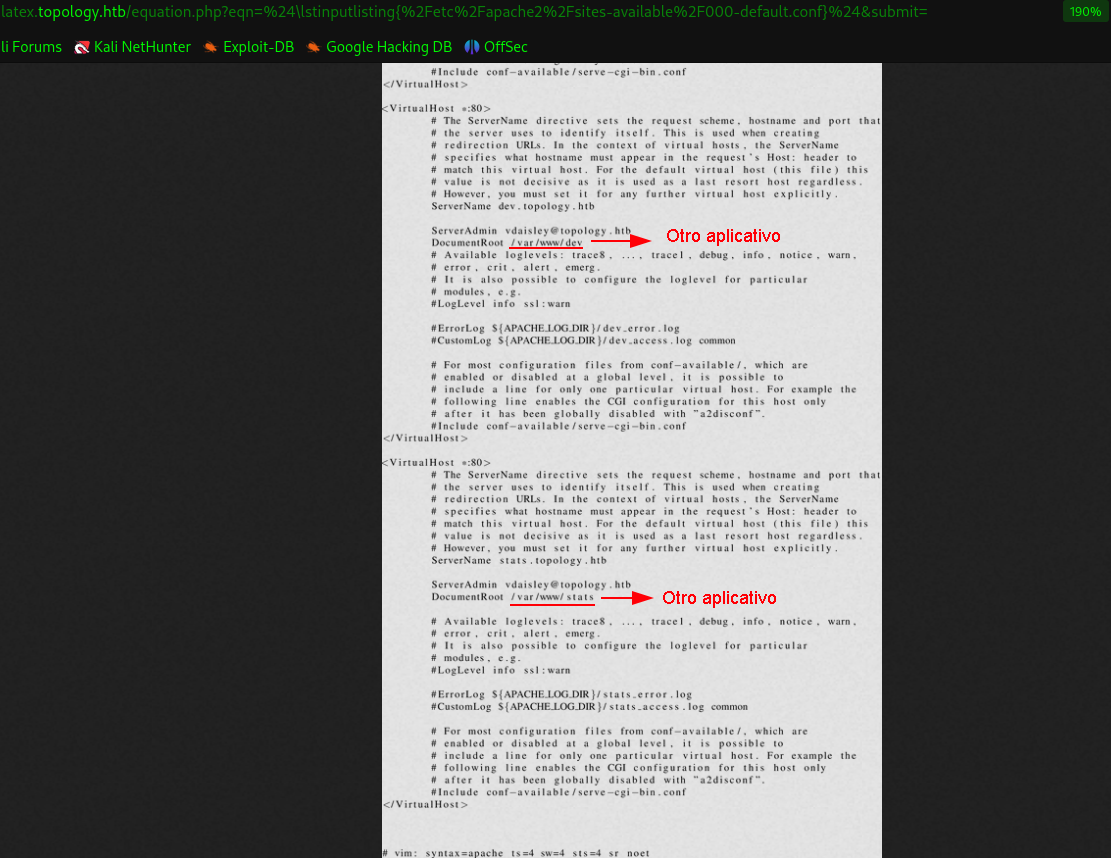
\includegraphics[width=1\textwidth]{images/otro-aplicativo.png}} % Utilizo \fbox para crear un borde alrededor de la imagen
        \end{center}
        \captionsetup{labelfont=bf} % Caption de la tabla en color negrita
        \caption{Nuevos aplicativos con sus respectivas rutas.}
    \end{figure}

    Para ingresar a los subdominios encontrados, debemos nuevamente agregarlos al archivo \textbf{/etc/hosts}

    \captionsetup[lstlisting]{labelfont=bf} % Caption del código en color negrita
    \begin{lstlisting}[language=c, caption=Agregando subdominios al archivo /etc/hosts, aboveskip=0.5cm]
        
    sudo nano /etc/hosts
          
    10.129.16.121 latex.topology.htb dev.topology.htb stats.topology.htb
    \end{lstlisting}

    \vspace{6cm}

    Lo único interesante es el subdominio \textbf{dev.topology.htb}, que tiene un formulario de login, pero no podemos ingresar por falta de credenciales.

    \begin{figure}[h] % Con "h" indico que coloque la imagen abajo del texto
        \begin{center}
        \setlength{\fboxsep}{0.2em} % Ajustar la distancia del borde interno
        \fbox{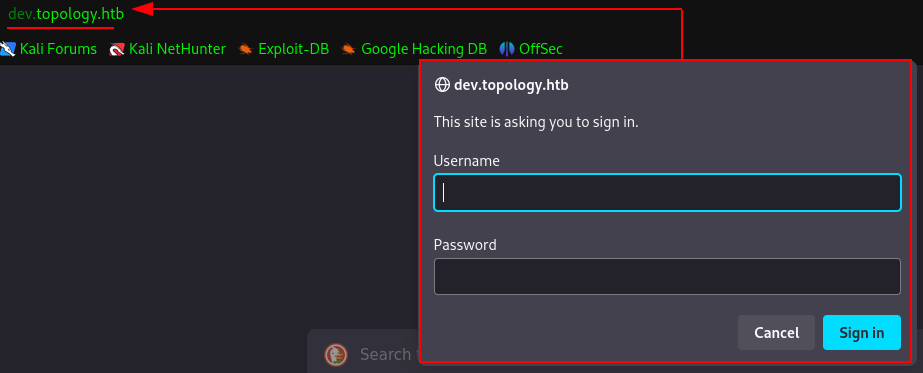
\includegraphics[width=1\textwidth]{images/dev-form-login.png}} % Utilizo \fbox para crear un borde alrededor de la imagen
        \end{center}
        \captionsetup{labelfont=bf} % Caption de la tabla en color negrita
        \caption{Fomrulario de inicio de sesión.}
    \end{figure}

    \vspace{15cm}

    Nuevamente utilizaremos el LFI para acceder al archivo \textbf{.htpasswd}, donde se supone que se guardan las credenciales de autenticación del servidor HTTP Apache.

    \begin{figure}[h] % Con "h" indico que coloque la imagen abajo del texto
        \begin{center}
        \setlength{\fboxsep}{0.2em} % Ajustar la distancia del borde interno
        \fbox{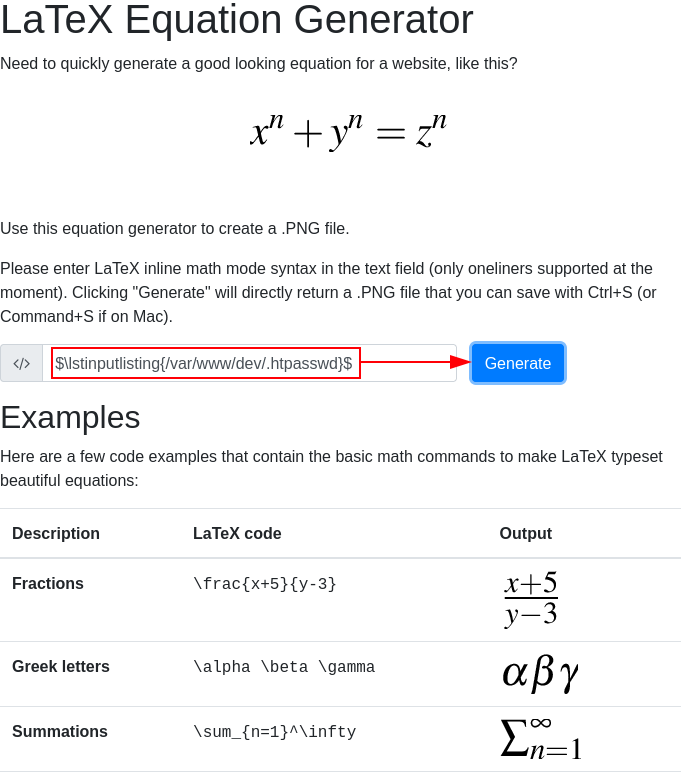
\includegraphics[width=0.9\textwidth]{images/lfi-htpasswd.png}} % Utilizo \fbox para crear un borde alrededor de la imagen
        \end{center}
        \captionsetup{labelfont=bf} % Caption de la tabla en color negrita
        \caption{LFI para el archivo .htpasswd}
    \end{figure}

    \vspace{5cm}

    Como resultado obtenemos un usuario y una contraseña cifrada, aparentemente con el \textbf{algoritmo} de \textbf{hashing} que usa \textbf{Apache} por defecto, que es \textbf{APR1}.

    \begin{figure}[h] % Con "h" indico que coloque la imagen abajo del texto
        \begin{center}
        \setlength{\fboxsep}{0.2em} % Ajustar la distancia del borde interno
        \fbox{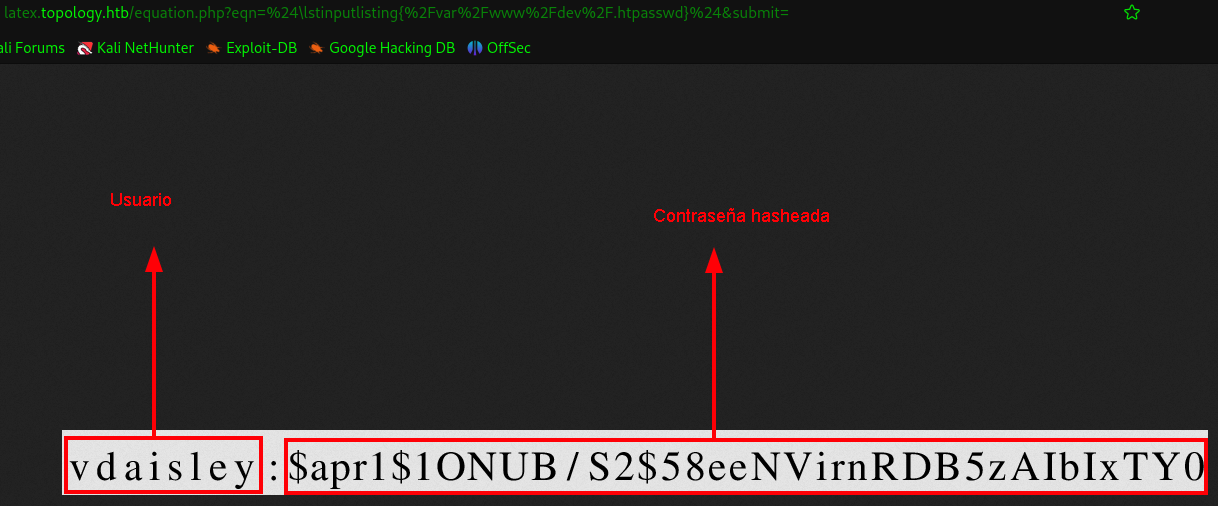
\includegraphics[width=1\textwidth]{images/user-passwd.png}} % Utilizo \fbox para crear un borde alrededor de la imagen
        \end{center}
        \captionsetup{labelfont=bf} % Caption de la tabla en color negrita
        \caption{Usuario y contraseña cifrada.}
    \end{figure}

    \subsection{Uso de la Herramienta John the Ripper}
    
    \vspace{0.2cm}

    Con el uso de la herramienta \href{https://www.kali.org/tools/john}{\textbf{\color{black}John the Ripper}} desciframos la contraseña.

    \begin{figure}[h] % Con "h" indico que coloque la imagen abajo del texto
        \begin{center}
        \setlength{\fboxsep}{0.2em} % Ajustar la distancia del borde interno
        \fbox{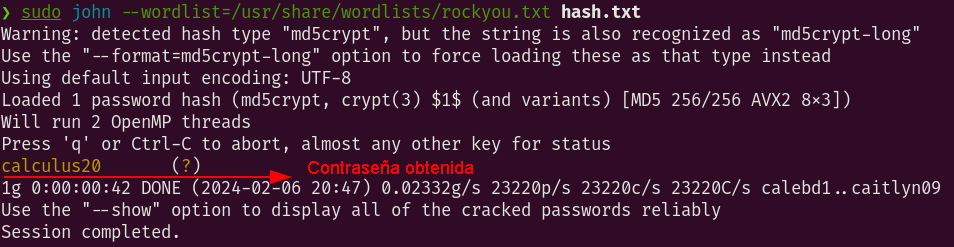
\includegraphics[width=1\textwidth]{images/passwd-deshasheda.png}} % Utilizo \fbox para crear un borde alrededor de la imagen
        \end{center}
        \captionsetup{labelfont=bf} % Caption de la tabla en color negrita
        \caption{Contraseña descifrada.}
    \end{figure}

    \vspace{9cm}

    La contraseña obtenida es \textbf{calculus20} y la utilizaremos en el formulario de login junto al usuario \textbf{vdaisley} que obtuvimos anteriormente.

    \begin{figure}[h] % Con "h" indico que coloque la imagen abajo del texto
        \begin{center}
        \setlength{\fboxsep}{0.2em} % Ajustar la distancia del borde interno
        \fbox{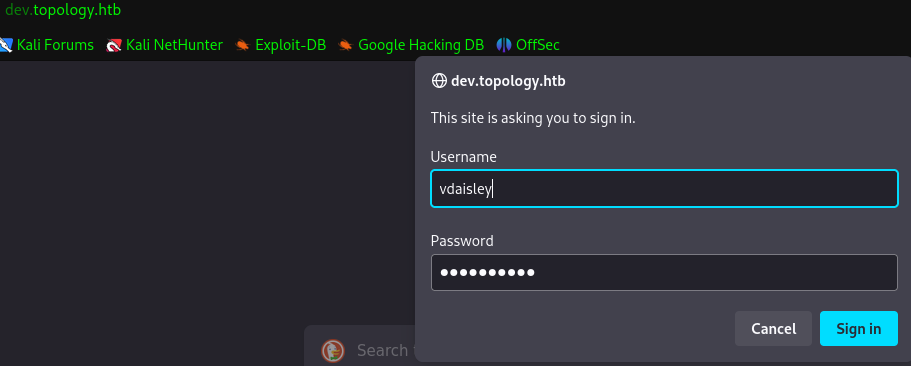
\includegraphics[width=0.9\textwidth]{images/creds-form-login.png}} % Utilizo \fbox para crear un borde alrededor de la imagen
        \end{center}
        \captionsetup{labelfont=bf} % Caption de la tabla en color negrita
        \caption{Iniciando sesión.}
    \end{figure}

    Al entrar no encontramos nada interesante, solo un software desarrollado por el personal de la \textbf{universidad Miskatonic}.

    \begin{figure}[h] % Con "h" indico que coloque la imagen abajo del texto
        \begin{center}
        \setlength{\fboxsep}{0.2em} % Ajustar la distancia del borde interno
        \fbox{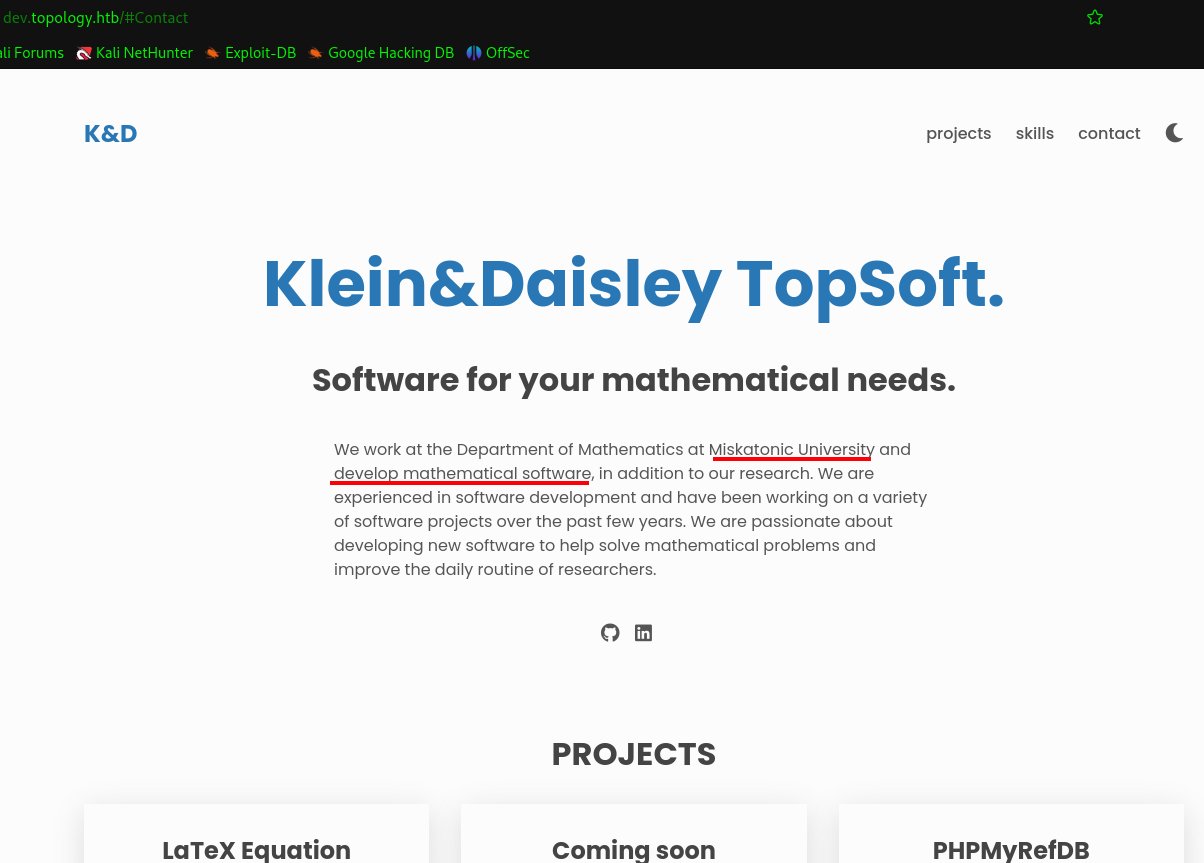
\includegraphics[width=0.8\textwidth]{images/dev-pag.png}} % Utilizo \fbox para crear un borde alrededor de la imagen
        \end{center}
        \captionsetup{labelfont=bf} % Caption de la tabla en color negrita
        \caption{Software desarrollado por el personal de la universidad.}
    \end{figure}

    \vspace{4cm}

    \subsection{Acceso al Sistema via SSH}
    
    \vspace{0.2cm}

    Al haber escaneado los puertos anteriormente y obtener información de que el puerto 22 que corresponde al servicio SSH esta abierto, procedemos a conectarnos por dicho servicio, utilizando las credenciales obtenidas.

    Al conectarnos exitosamente, podemos leer la \textcolor{blue}{flag} del \textbf{user}. 

    \begin{figure}[h] % Con "h" indico que coloque la imagen abajo del texto
        \begin{center}
        \setlength{\fboxsep}{0.2em} % Ajustar la distancia del borde interno
        \fbox{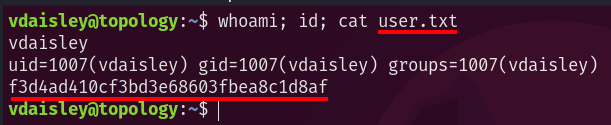
\includegraphics[width=1\textwidth]{images/user-flag.png}} % Utilizo \fbox para crear un borde alrededor de la imagen
        \end{center}
        \captionsetup{labelfont=bf} % Caption de la tabla en color negrita
        \caption{Conexión por SSH.}
    \end{figure}

    \subsection{Listamiento de Directorios Interesantes}
    
    \vspace{0.2cm}

    Una vez dentro, vemos en el directorio \textbf{opt} que se encuentra un directorio llamado \textbf{gnuplot}, el cual tiene permisos de \textbf{escritura} y \textbf{ejecución}, y cuyo propietario es \textbf{root}.

    \begin{figure}[h] % Con "h" indico que coloque la imagen abajo del texto
        \begin{center}
        \setlength{\fboxsep}{0.2em} % Ajustar la distancia del borde interno
        \fbox{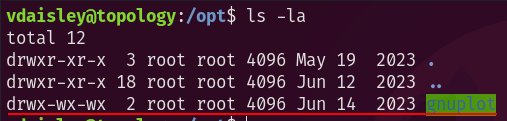
\includegraphics[width=1\textwidth]{images/gnuplot.png}} % Utilizo \fbox para crear un borde alrededor de la imagen
        \end{center}
        \captionsetup{labelfont=bf} % Caption de la tabla en color negrita
        \caption{Directorio opt.}
    \end{figure}

    Investigando un poco encontre que \textbf{gnuplot} es un programa de interfaz de línea de comandos para generar gráficas de dos y tres dimensiones de funciones, datos y ajustes de datos.

\vspace{6cm}

\section{Escalada de Privilegios}

    \subsection{Uso de la Herramienta pspy}

    \vspace{0.2cm}

    Para seguir enumernado la máquina victima utilizaré \href{https://github.com/DominicBreuker/pspy}{\textbf{\color{black}pspy}}, que es una herramienta de monitoreo de procesos para sistemas Linux. Esta herramienta permitira enumerar procesos de la máquina victima.

    Antes debo saber cuál es la arquitectura y la cantidad de bits del sistema Linux de la máquina víctima, para poder descargar el ejecutable de pspy para la arquitectura correspondiente.

    Para eso ejecuto el comando \textbf{uname -m}, en el cual obtengo que la arquitectura de la máquina victima es de 64 bits.

    \begin{figure}[h] % Con "h" indico que coloque la imagen abajo del texto
        \begin{center}
        \setlength{\fboxsep}{0.2em} % Ajustar la distancia del borde interno
        \fbox{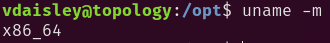
\includegraphics[width=1\textwidth]{images/64-bits.png}} % Utilizo \fbox para crear un borde alrededor de la imagen
        \end{center}
        \captionsetup{labelfont=bf} % Caption de la tabla en color negrita
        \caption{Arquitectura de 64 Bits.}
    \end{figure}

    Una vez teniendo este dato me descargo el ejecutable de pspy y creo en el servidor python en el puerto 80, para luego desde la máquina victima realizar una petición wget y pasarme el archivo de la herramienta.

    Realizamos una petición wget en la máquina victima.

    \begin{figure}[h] % Con "h" indico que coloque la imagen abajo del texto
        \begin{center}
        \setlength{\fboxsep}{0.2em} % Ajustar la distancia del borde interno
        \fbox{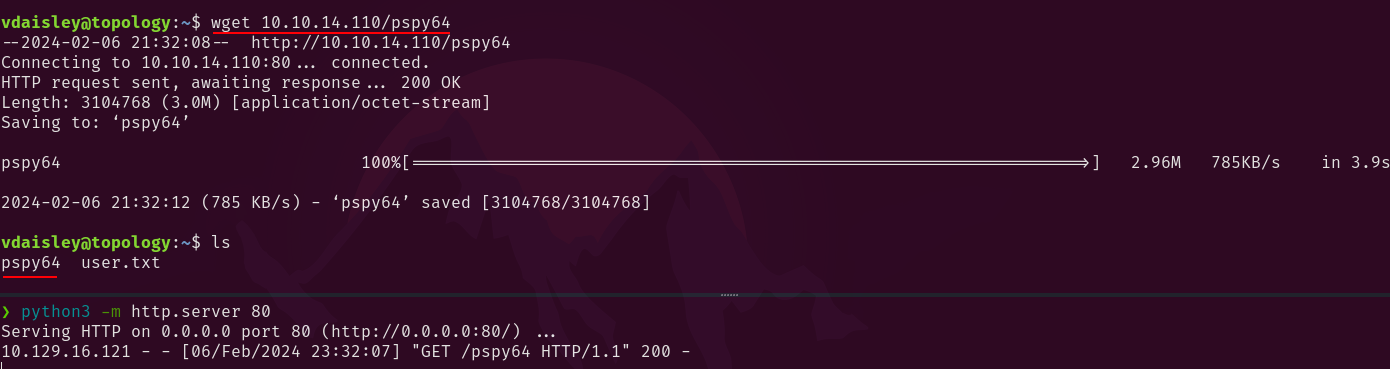
\includegraphics[width=1\textwidth]{images/wget.png}} % Utilizo \fbox para crear un borde alrededor de la imagen
        \end{center}
        \captionsetup{labelfont=bf} % Caption de la tabla en color negrita
        \caption{Petición wget.}
    \end{figure}

    \vspace{9cm}

    Le asignamos permisos de ejecución al ejecutable de pspy.

    \begin{figure}[h] % Con "h" indico que coloque la imagen abajo del texto
        \begin{center}
        \setlength{\fboxsep}{0.2em} % Ajustar la distancia del borde interno
        \fbox{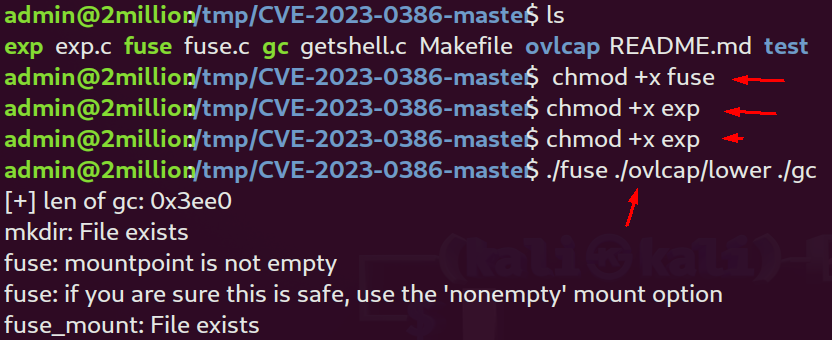
\includegraphics[width=1\textwidth]{images/chmod.png}} % Utilizo \fbox para crear un borde alrededor de la imagen
        \end{center}
        \captionsetup{labelfont=bf} % Caption de la tabla en color negrita
        \caption{Asignando permisos de ejecución.}
    \end{figure}

    Una vez asignados los permisos de ejecución, procedemos a ejecutarlo y observamos que el usuario con \textbf{UID=0}, o sea el usuario \textbf{root}, ejecuta el comando \textbf{find} sobre el directorio \textbf{/opt/gnuplot}, donde busca todos los archivos con extensión \textbf{.plt} (que es la extensión que corresponde al programa gnuplot) y luego los ejecuta.

    Luego ejecuta una serie de scripts y por ultimo ejecuta un archivo \textbf{networkplot.plt}

    \begin{figure}[h] % Con "h" indico que coloque la imagen abajo del texto
        \begin{center}
        \setlength{\fboxsep}{0.2em} % Ajustar la distancia del borde interno
        \fbox{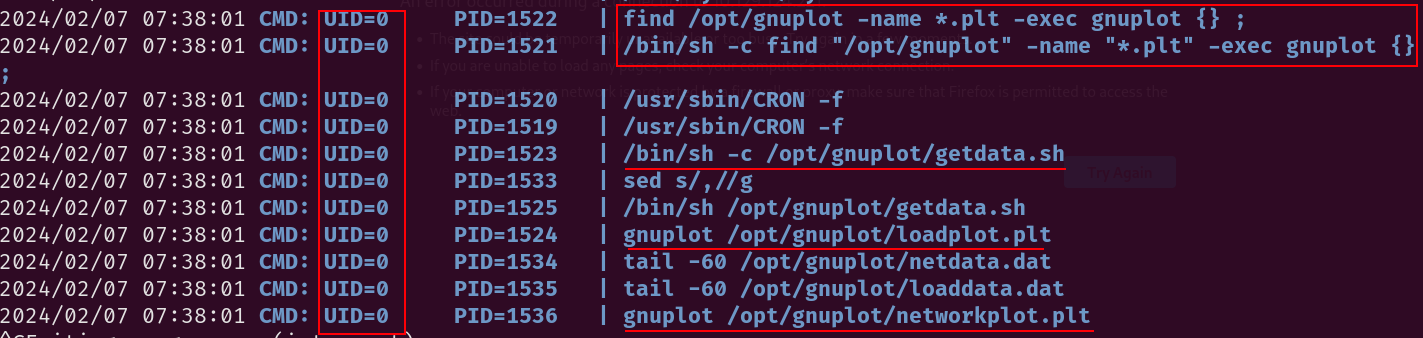
\includegraphics[width=1\textwidth]{images/resultado-pspy.png}} % Utilizo \fbox para crear un borde alrededor de la imagen
        \end{center}
        \captionsetup{labelfont=bf} % Caption de la tabla en color negrita
        \caption{Procesos.}
    \end{figure}

    Nos damos cuenta en el directorio \textbf{/opt/gnuplot} tenemos permisos de escritura pero no de listamiento.

    \begin{figure}[h] % Con "h" indico que coloque la imagen abajo del texto
        \begin{center}
        \setlength{\fboxsep}{0.2em} % Ajustar la distancia del borde interno
        \fbox{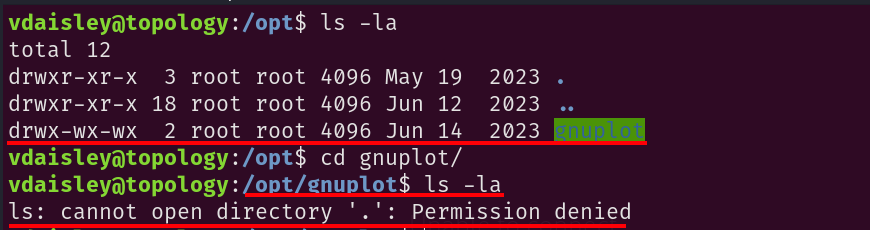
\includegraphics[width=1\textwidth]{images/permisos.png}} % Utilizo \fbox para crear un borde alrededor de la imagen
        \end{center}
        \captionsetup{labelfont=bf} % Caption de la tabla en color negrita
        \caption{Permisos.}
    \end{figure}

    \vspace{9cm}

    \subsection{Creación del Exploit}

    \vspace{0.2cm}

    Lo que se me ocurre es crear un archivo asignando permisos \textbf{SUID} para convertir la \textbf{BASH} del sistema, de modo que luego root ejecute el script habilitando el \textbf{Bit SUID} y enlace una BASH con altos privilegios.

    \captionsetup[lstlisting]{labelfont=bf} % Caption del código en color negrita
    \begin{lstlisting}[caption=Exploit., aboveskip=0.5cm]
        
    nano root.plt
          
    system "chmod u+s /bin/bash"
    \end{lstlisting}

    Una vez creado el archivo, ejecutamos de vuelta pspy para saber cuando root ejecuto el archivo.

    \begin{figure}[h] % Con "h" indico que coloque la imagen abajo del texto
        \begin{center}
        \setlength{\fboxsep}{0.2em} % Ajustar la distancia del borde interno
        \fbox{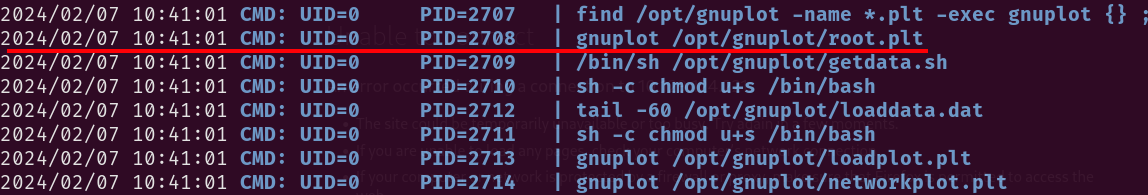
\includegraphics[width=1\textwidth]{images/pspy-script.png}} % Utilizo \fbox para crear un borde alrededor de la imagen
        \end{center}
        \captionsetup{labelfont=bf} % Caption de la tabla en color negrita
        \caption{Archivo ejecutado.}
    \end{figure}

    Para confirmar hacemos un \textbf{ls -la} de la bash y vemos que tiene el Bit SUID activado.

    \begin{figure}[h] % Con "h" indico que coloque la imagen abajo del texto
        \begin{center}
        \setlength{\fboxsep}{0.2em} % Ajustar la distancia del borde interno
        \fbox{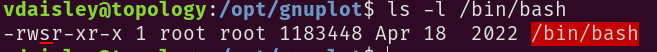
\includegraphics[width=1\textwidth]{images/ls-l-bash.png}} % Utilizo \fbox para crear un borde alrededor de la imagen
        \end{center}
        \captionsetup{labelfont=bf} % Caption de la tabla en color negrita
        \caption{Bit SUID activado.}
    \end{figure}

    Simplemente ahora hacemos \textbf{bash -p} y conseguimos escalar privilegios y obtener la \textcolor{red}{flag} de \textbf{root}.

    \begin{figure}[h] % Con "h" indico que coloque la imagen abajo del texto
        \begin{center}
        \setlength{\fboxsep}{0.2em} % Ajustar la distancia del borde interno
        \fbox{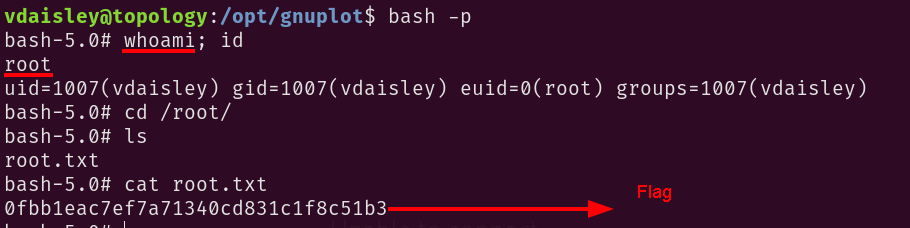
\includegraphics[width=1\textwidth]{images/whoami-flag.png}} % Utilizo \fbox para crear un borde alrededor de la imagen
        \end{center}
        \captionsetup{labelfont=bf} % Caption de la tabla en color negrita
        \caption{Flag.}
    \end{figure}

\vspace{5cm}

\section{Conclusión Final}

Esta máquina resultó muy entretenida, ideal para aquellos que recién comienzan en el pentesting resolviendo máquinas. La verdad es que fue bastante sencilla, en mi caso nunca había explorado ni explotado un Local File Inclusion (LFI) a través LaTeX Injection. Si no fuera por eso, la habría terminado antes. Después de eso, la parte de explotación y priv-esc no me dio problemas.

\section{Apéndice I Links de Referencia}

    \subsection{Herramientas Utilizadas en la Auditoria}

    \begin{itemize}
        \item \href{https://nmap.org}{\textbf{\color{black}Nmap}}: \href{https://nmap.org}{\textbf{\color{blue}https://nmap.org}} - \href{https://www.kali.org/tools/nmap}{\textbf{\color{blue}https://www.kali.org/tools/nmap}} \texttt{{-}{-}{-}>} Uso de nmap para el escaneo de puertos.
        \item \href{https://www.openwall.com/john}{\textbf{\color{black}John the Ripper}}: \href{https://www.openwall.com/john}{\textbf{\color{blue}https://www.openwall.com/john}} - \href{https://www.kali.org/tools/john}{\textbf{\color{blue}https://www.kali.org/tools/john}}
    \end{itemize}
    \hspace{1cm} - \href{https://github.com/openwall/john}{\textbf{\color{blue}https://github.com/openwall/john}} \texttt{{-}{-}{-}>} Uso de John the Ripper para descifrar contraseña.
    \begin{itemize}
        \item \href{https://github.com/DominicBreuker/pspy}{\textbf{\color{black}pspy - unprivileged Linux process snooping}}: \href{https://github.com/DominicBreuker/pspy}{\textbf{\color{blue}https://github.com/DominicBreuker/pspy}} \texttt{{-}{-}{-}>} Uso de pspy para monitorear procesos.
    \end{itemize}
        
    \subsection{Documentación}

    \begin{itemize}
        \item \href{https://book.hacktricks.xyz/pentesting-web/formula-csv-doc-latex-ghostscript-injection}{\textbf{\color{black}HackTricks: LaTeX Injection}} \href{https://book.hacktricks.xyz/pentesting-web/formula-csv-doc-latex-ghostscript-injection}{\textbf{\color{blue}https://book.hacktricks.xyz/pentesting-web/formula-csv-doc-latex-ghostscript-injection}}
        \item \href{https://exploit-notes.hdks.org/exploit/linux/privilege-escalation/gnuplot-privilege-escalation}{\textbf{\color{black}Gnuplot Privilege Escalation}}:
    \end{itemize}

    \hspace{1cm}\href{https://exploit-notes.hdks.org/exploit/linux/privilege-escalation/gnuplot-privilege-escalation}{\textbf{\color{blue}https://exploit-notes.hdks.org/exploit/linux/privilege-escalation/gnuplot-privilege-escalation}}
    
\section{Contacto}

\begin{minipage}{0.05\textwidth}
  
\includegraphics[width=0.7\textwidth]{images/gmail.png} 
\end{minipage}
\begin{minipage}{.7\textwidth}
    \vspace{1mm} % Ajusta este valor según sea necesario para subir o bajar el bloque de texto
    \href{mailto:marianoalfonso80@protonmail.com}{\textbf{\color{black}E-mail}}: \href{mailto:marianoalfonso80@protonmail.com}{\textbf{\color{blue}marianoalfonso80@protonmail.com}}
\end{minipage} 

\begin{minipage}{0.05\textwidth}
    
\includegraphics[width=0.7\textwidth]{images/linkedin.png} 
\end{minipage}
\begin{minipage}{.7\textwidth}
    \vspace{1mm} % Ajusta este valor según sea necesario para subir o bajar el bloque de texto
    \href{https://www.linkedin.com/in/mariano-alfonso-667a60226}{\textbf{\color{black}LinkedIn}}: \href{https://www.linkedin.com/in/mariano-alfonso-667a60226}{\textbf{\color{blue}https://www.linkedin.com/in/mariano-alfonso-667a60226}}
\end{minipage} 

\begin{minipage}{0.05\textwidth}
    
\includegraphics[width=0.7\textwidth]{images/im_maa.png} 
\end{minipage}
\begin{minipage}{.7\textwidth}
    \vspace{1mm} % Ajusta este valor según sea necesario para subir o bajar el bloque de texto
    \href{https://0mariano.github.io}{\textbf{\color{black}Blog}}: \href{https://0mariano.github.io}{\textbf{\color{blue}https://0mariano.github.io}}
\end{minipage}

\begin{minipage}{0.05\textwidth}
    
\includegraphics[width=0.7\textwidth]{images/github.png} 
\end{minipage}
\begin{minipage}{.7\textwidth}
    \vspace{1mm} % Ajusta este valor según sea necesario para subir o bajar el bloque de texto
    \href{https://github.com/0mariano}{\textbf{\color{black}GitHub}}: \href{https://github.com/0mariano}{\textbf{\color{blue}https://github.com/0mariano}}
\end{minipage}

\end{document}